\documentclass[12pt]{article}

\usepackage{fontawesome}
\usepackage{hyperref}
\usepackage{xurl}
\usepackage{graphicx}
\usepackage{float}
\usepackage[tagged, highstructure]{accessibility}
\usepackage{bookmark}
\usepackage{enumitem}

\hypersetup{
    colorlinks=false,
    pdfborder={0 0 0},
    pdftitle={SQL Review Part 2},
    pdfauthor={Adrianna Holden-Gouveia},
    pdfsubject={Advanced Data - Lab Assignment},
    pdflang={en-US},
    pdfkeywords={SQL, table joins, relationships, HackerRank, advanced SQL}
}

% Configure PDF bookmarks for navigation
\bookmarksetup{
    numbered,
    open,
}

% Configure list spacing for better accessibility
\setlist{nosep}



\title{SQL Review Part 2}
\author{
        Adrianna Holden-Gouveia \\
        Website: \href{https://aholdengouveia.name}{aholdengouveia.name}\\ 
        \date{\vspace{-5ex}}
        %Email: \href{mailto:admin@aholdengouveia.name}{admin@aholdengouveia.name} \\
%        \faLinkedin{: aholdengouveia} \\
        \faGithub {: aholdengouveia} \\
        %\faTwitter {: aholdengouveia} \\
        }

%S\date{\today}


\begin{document}    

\maketitle

%\begin{abstract}
%This is a template for Linux Administration Lab work
%\end{abstract}
%\tableofcontents


\section*{Accessibility Notice}
This document is also available in HTML format at:

Link: \href{https://aholdengouveia.name/AdvData/labs/week3.html}{\textbf{\nolinkurl{https://aholdengouveia.name/AdvData/labs/week3.html}}}

The HTML version provides enhanced accessibility features including keyboard navigation, screen reader support, responsive design, dark mode support, and high contrast options.

\section*{Request}
\noindent\textbf{Request:} DATA-5809\\
\textbf{Requested by:} Inventory lead\\
\textbf{Data:} Your database from the SQL Review lab

\section*{Background}
Your manager liked your first queries. Now the inventory lead wants to combine your data with a second table, and to know whether anything in the data doesn't match up. Rows that don't match are a common sign of data problems, and finding them early saves the company time and money. You'll start with join training, then apply it to your own data.

\section*{Learning Outcomes}
By the end of this lab, you will be able to:
\begin{itemize}
    \item Write SQL queries that join two tables
    \item Create a lookup table, and explain how it relates to your data using primary and foreign keys
    \item Choose between an inner join and a left join, and explain how the results differ
    \item Use a join to find data quality problems, such as rows with no match
\end{itemize}

\section*{Lab Instructions}

\subsection*{Screenshots}
Several parts of this lab ask for a screenshot. Each screenshot should have your name, term, and year.  One of the easiest ways to do that is make a text document with your name and term/year on your computer and save it to use all term. Any screenshots that don't include this information won't be counted.

\begin{figure}[H]
    \centerline{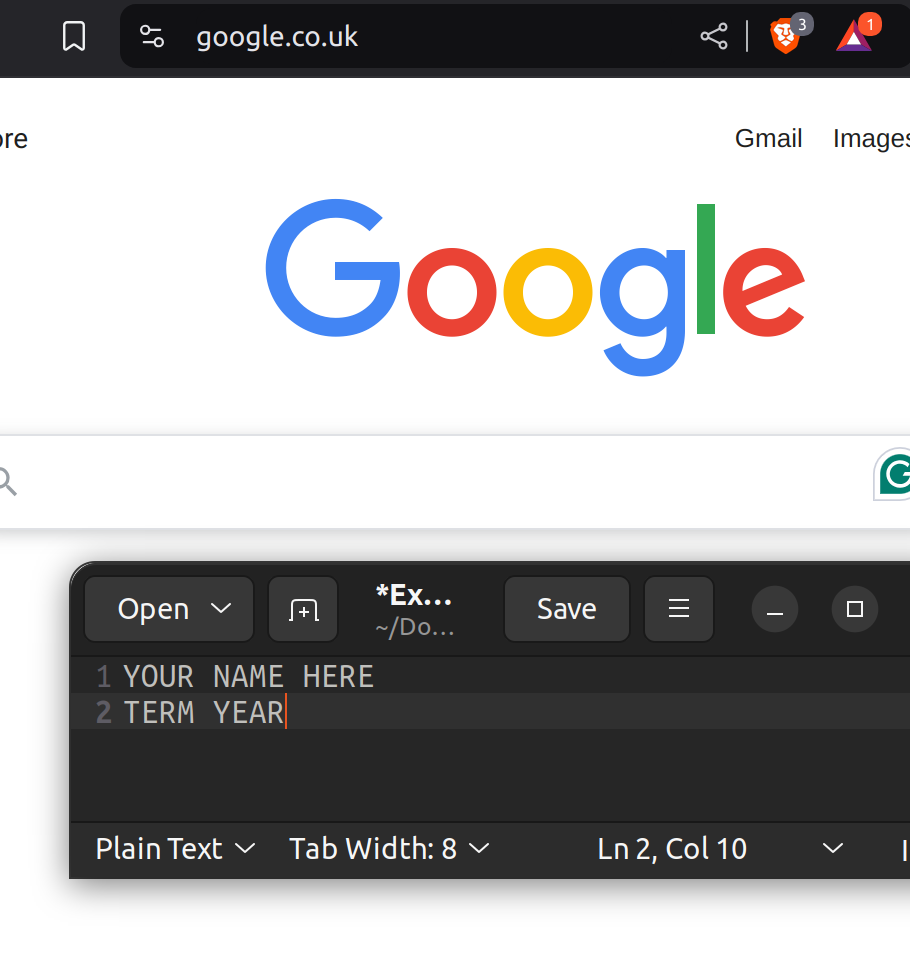
\includegraphics[scale=.2]{ExampleScreenshot.png}}
    \caption{This is an image of what each of your screenshots should look like}
    \alt{Example screenshot: a web browser showing the Google home page, with a small text editor window in front of it that says YOUR NAME HERE and TERM YEAR}
\end{figure}

\subsection*{Part 1: SQL Joins Tutorial}
Go through these 3 sections of SQLBolt (linked under Resources), and complete the exercises at the end of each one:
\begin{itemize}
    \item SQL Lesson 6: Multi-table queries with JOINs
    \item SQL Lesson 7: OUTER JOINs
    \item SQL Lesson 8: A short note on NULLs
\end{itemize}
Take a screenshot of each section after you complete its exercises. Make sure you have the green checkmark on each problem.

\subsection*{Part 2: Join Challenges}
Complete 3 HackerRank challenges that use joins (linked under Resources). You can filter the list by basic and advanced joins. HackerRank is free, but you need to register so your work is saved to your profile.
\begin{enumerate}
    \item Take a screenshot of each solution.
    \item With each screenshot, explain how you solved it and what resources you used. If you needed a hint, say where you found it.
    \item Pick one of your 3 solutions and explain which type of join you used and why. What would change in the results if you used the other type (inner instead of left, or left instead of inner)?
    \item Take a screenshot of your HackerRank profile showing the completed challenges.
\end{enumerate}
\textbf{Optional, not required for this class:} if you'd like more practice, try more of the HackerRank join challenges.

\subsection*{Part 3: Joins on Your Data}
Your data set from the SQL Review lab is one table, so you'll make a second table to join it to. Books are my example data only, so use your own data set.
\begin{enumerate}
    \item Create a small lookup table with 5 to 10 rows that adds information about one column in your main table. For example, my book data has a format column, so I made a table that matches each format to the shelf section where it goes in the store.
    \item Explain how the two tables relate. Which column links them? What is the primary key of your lookup table, and which column in your main table acts as the foreign key?
    \item Write 3 queries that join your two tables, documented in the same format as the SQL Review lab. Use at least one inner join and at least one left join.
    \item Make one of your 3 queries a data quality check: use a left join to find rows in your main table that have no match in your lookup table. In the Notes, explain why those rows don't match and what you would do about it.
    \item Take a screenshot of each query and its results.
\end{enumerate}

\section*{Acceptance Criteria}
This request is done when:
\begin{itemize}
    \item All 3 SQLBolt sections are complete, with a green checkmark on every problem
    \item 3 HackerRank join challenges are solved, each with an explanation, and your profile shows them complete
    \item Your lookup table has 5 to 10 rows and a primary key, and you've explained how it links to your main table
    \item 3 join queries documented in the sample format, with at least one inner join and one left join
    \item One query is a data quality check, with notes explaining the rows that don't match and what to do about them
    \item Every screenshot follows the screenshot rules
\end{itemize}

\section*{Deliverables}
One file that includes:
\begin{itemize}
    \item Part 1: your 3 SQLBolt screenshots
    \item Part 2: your 3 HackerRank screenshots with explanations, your answer about join types, and your profile screenshot
    \item Part 3: the commands you used to create your lookup table, your explanation of how the tables relate, and your 3 documented queries with a screenshot of each one and its results
\end{itemize}

Audience: the inventory lead and the rest of the data team.

\section*{Resources}
References, a video, a PowerPoint and some notes are available at my website
Link: \href{https://www.aholdengouveia.name/AdvData/sqlpt2.html}{\textbf{\nolinkurl{https://www.aholdengouveia.name/AdvData/sqlpt2.html}}}

SQLBolt, the tutorial for Part 1
Link: \href{https://sqlbolt.com/}{\textbf{\nolinkurl{https://sqlbolt.com/}}}

HackerRank join challenges for Part 2
Link: \href{https://www.hackerrank.com/domains/sql?filters%5Bsubdomains%5D%5B%5D=join&filters%5Bsubdomains%5D%5B%5D=advanced-join}{\textbf{\nolinkurl{https://www.hackerrank.com/domains/sql?filters\%5Bsubdomains\%5D\%5B\%5D=join&filters\%5Bsubdomains\%5D\%5B\%5D=advanced-join}}}

Sample query documentation, with join examples (Q3 and Q4)
Link: \href{https://www.aholdengouveia.name/AdvData/labs/SampleQueryDocumentation.txt}{\textbf{\nolinkurl{https://www.aholdengouveia.name/AdvData/labs/SampleQueryDocumentation.txt}}}

\end{document}